%! Author = t.kramer
%! Date = 15/09/2024

\section{Research context}

% Research context
Indoor thermal comfort is strongly associated with occupant well-being \citep{altomonte_ten_2020}, overall satisfaction \citep{graham_lessons_2021} and energy use in buildings \citep{yang_thermal_2014}. As such, accurately projecting operational thermal comfort is a critical aspect of early building design.

% Overview of current metrics
In the traditional design workflow, thermal comfort assessments rely heavily on simulation data. This data forms the basis for calculating hourly thermal comfort indices, e.g., the Predicted Mean Vote (PMV). This indices are then aggregated into an annual, single-value metric \Cref{fig:typical-workflow}. Common long-term metrics derived from this approach include the \textit{Percentage of Time Outside a PMV} or \textit{Operative Temperature Range} (as outlined by ISO, EN, and ASHRAE standards) and the \textit{Degree Hours} method. Such metrics provide a broad, building-wide assessment of thermal comfort and are instrumental in guiding key design decisions regarding building form, envelope and particularly HVAC system design.

\begin{figure*}[h!]
    \centering
    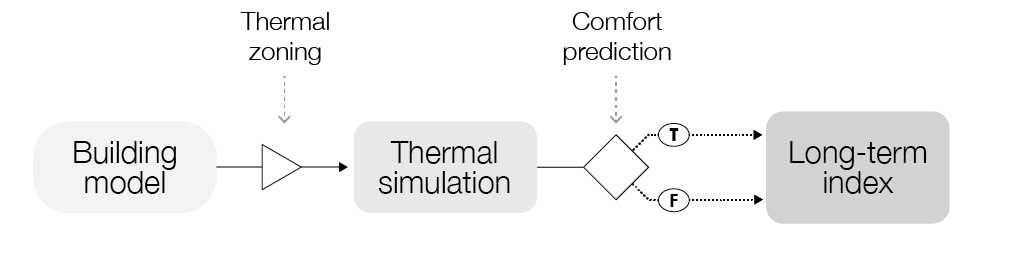
\includegraphics[width=8.9cm]{manuscript/src/figures/conventional-workflow.png}
    \caption{Traditional long-term thermal comfort prediction: Hourly simulated indoor climate data is assessed using thermal comfort index (e.g. PMV) and is aggregated into a single value long-term (e.g. annual) metric. }
    \label{fig:typical-workflow}
\end{figure*}

% Critique 
Despite their widespread use, these traditional thermal comfort metrics have inherent limitations. For instance, \citet{li_improved_2020} found that many of these metrics, including those established in industry standards, show a weak correlation with actual thermal satisfaction among occupants.

Another significant issue is that most long-term metrics featured in standards rely on the Predicted Mean Vote (PMV) index. Recent research has highlighted several shortcomings of the PMV index: it often exhibits poor predictive accuracy \citep{cheung_analysis_2019}, advocates for excessively narrow temperature ranges \citep{arens_are_2010}, and depends on personal factors such as clothing insulation and metabolic activity \citep{gauthier_role_2013}—variables that are inherently unpredictable and often treated as constants in models \citep{carlucci_review_2012}, thus failing to represent real-world behavior accurately. This reliance on rigid assumptions frequently leads to the promotion of overly tight temperature controls, which in turn drives unnecessary energy consumption for space conditioning \citep{fukawa_field_2021, sekhar_thermal_2016}.

Furthermore, conventional metrics typically capture only the temporal variability of thermal comfort, overlooking the spatial differences within a thermal zone. This is a significant oversight, as recent studies have identified pronounced spatial thermal heterogeneity within indoor spaces \citep{mishra_thermal_2016, kramer_personal_2023}.

% Objective  
The objective of this paper is to introduce a new metric for comfort-based building performance assessment: spatial Thermal Autonomy (sTA). Compared to traditional metrics, sTA offers two significant advantages: (a) it accounts for spatial thermal variability, ensuring a more comprehensive evaluation of comfort throughout a building, and (b) it emphasizes energy-autonomous, passive building performance, reducing dependence on external energy sources.




